\section{Struktura danych CDLMW(s)}
\label{sec:cdlmw}
Struktura \textsc{CDLMW(s)} (algorytm 1 z pracy \cite{chan14}) jest modyfikacją struktury \textsc{KMS(s)}. Główną zmianą w porównaniu do struktury \textsc{KMS(s)} jest sposób w jaki obsługujemy prefiks i sufiks podczas operacji \textsc{query}. Dzięki tej zmianie pozbywamy się logarytmu w czasie operacji \textsc{query}. Analogicznie do struktury \textsc{KMS(s)} będziemy dzielić tablicę $A$ na $s$ bloków, każdy, prócz ostatniego, o rozmiarze $t=\cl{n/s}$. $i$-ty blok $B_i$ dla $i=0,1,\dots,s-1$ reprezentuje przedział $A[it+1, \min(n,(i+1)t)]$.
Struktura  \textsc{CDLMW(s)} wspiera następujące operacje dla statycznej tablicy $A[1:n]$:
\begin{enumerate}[nosep]
    \item \textsc{count}$(h,i,j)$ -- Oblicza $F^A_{A[i]}(i, j)$ w czasie $\Oh(F^A_{A[i]}(i, j) - h)$. Zakładamy, że $1 \le h \le F^A_{A[i]}(i,j).$
    \item \textsc{query}$(i, j)$ -- Oblicza dominantę i jej częstotliwość w czasie $\Oh(n/s)$.
\end{enumerate}
Parametr $h$ operacji \textsc{count}$(h,i,j)$ jest podpowiedzią ile razy co najmniej wartość $A[i]$ występuje w przedziale $A[i:j]$.
\subsection{Konstrukcja struktury \textsc{CDLMW(s)}}
\begin{figure}[H]
    \centering
    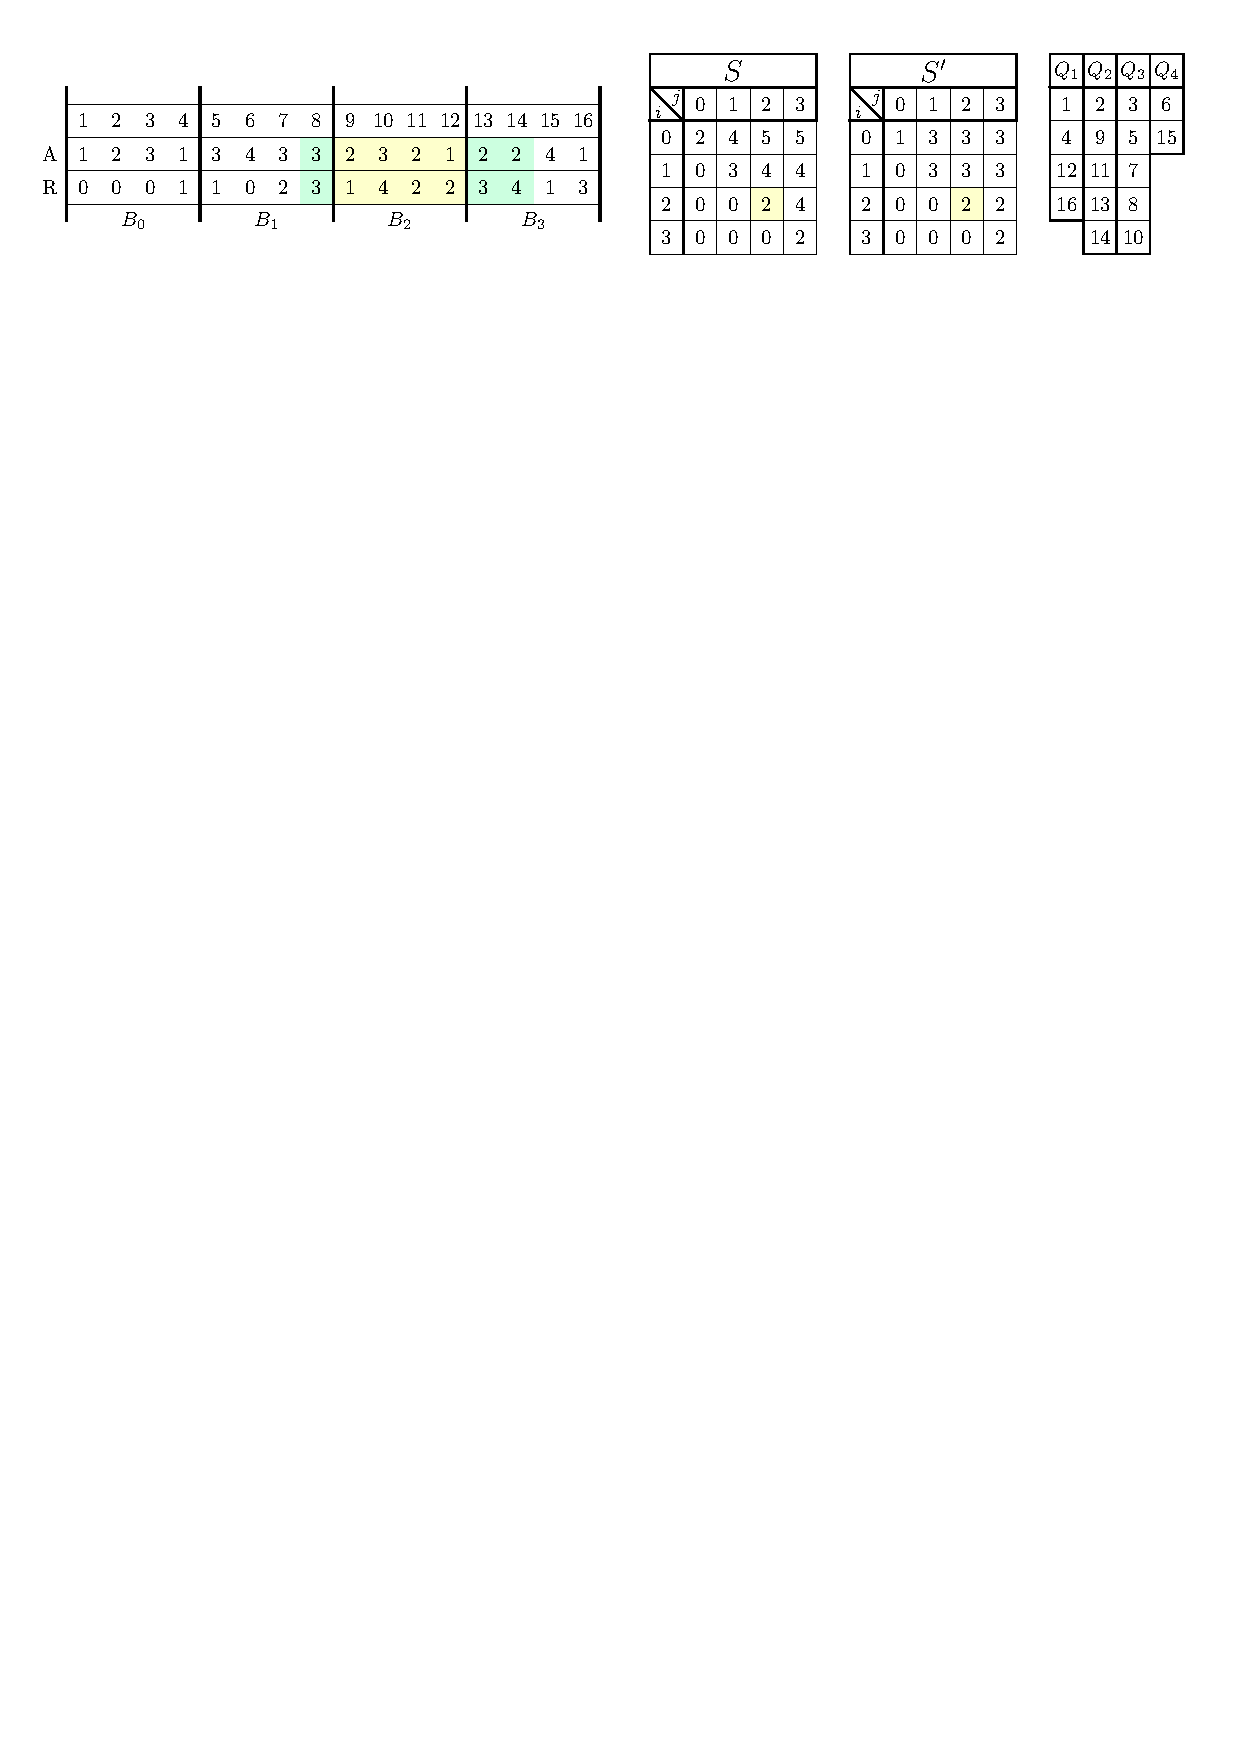
\includegraphics[scale=0.85]{images/cdlmw.pdf}
    \caption{Przykładowa tablica $A[1:16]$ z liczbą unikalnych elementów $\dt=4$ i podziałem na $s=4$ bloki, każdy o rozmiarze $t=4$. Ponadto zaznaczamy zapytanie o dominantę $A[8:14]$ z rozbiciem na prefiks $A[8:8]$, środek $A[9:12]$ oraz sufiks $A[13:14]$, które są zaznaczone odpowiednio kolorami zielonym, żółtym i zielonym.}
    \label{fig:cdlmw}
\end{figure}
Konstruujemy tablice S, S' oraz $\dt$ tablic $Q_x$, które są opisane przy konstrukcji struktury danych KMS. Ponadto konstruujemy jedną dodatkową tablicę $R[1:n]$, która na $i$-tej pozycji zawiera indeks wartości $A[i]$ w tablicy $Q_{A[i]}$. Równoważnie możemy zdefiniować $R$, aby spełniała taką własność: $Q_{A[i]}[R[i]] = i$.

\subsection{Operacja \textsc{count}}
\begin{algorithm}
    \caption{Operacja \textsc{count}}
    \label{alg:cdlmw-count}
    \begin{algorithmic}[1]
        \Function{count}{$h$,$i$,$j$}
            \State $l \gets R[i]$
            \State $m \gets R[i]+h$
            \While {$m < size(Q_{A[i]}) \land Q_{A[i]}[m] \le j$}
                \State $m \gets m + 1$
            \EndWhile
            \State \Return $m - l$
        \EndFunction
    \end{algorithmic}
\end{algorithm}
Załóżmy, że chcemy policzyć $F^A_{A[i]}(i,j)$, z dodatkową wiedzą, że element $A[i]$ występuje w przedziale $A[i:j]$ co najmniej $h$ razy. Wiemy, że wszystkie indeksy wystąpień $A[i]$ na przedziale $A[i:j]$ tworzą spójny fragment w tablicy $Q_{A[i]}$. Tablica $R$ umożliwia nam znalezienie początku tego fragmentu w czasie stałym. Moglibyśmy przeskanować liniowo ten fragment tablicy  $Q_{A[i]}$ i znaleźć wszystkie wystąpienia elementu $A[i]$ na przedziale $A[i:j]$. Jednakże dzięki podpowiedzi $h$ możemy to przyśpieszyć i ominąć pierwsze $h$ indeksów zaczynając od indeksu $R[i]$ w tablicy $Q_{A[i]}$. 

\subsection{Operacja \textsc{query}}
\begin{algorithm}[t]
    \caption{Operacja \textsc{query}}
    \label{alg:cdlmw-query}
    \begin{algorithmic}[1]
        \Function{query}{$i$,$j$}
            \State $b_i \gets \fl{(i-1)/t}$
            \State $b_j \gets \fl{(j-1)/t}$
            \State $mfreq \gets S'[b_i+1,b_j-1]$
            \State $mmode \gets S[b_i+1,b_j-1]$
            \For{k $\in$ prefiks $\cup$ sufiks}
                    \If{$R[k] = 0 \lor Q_{A[i]}[R[k]-1] < i$}
                        \If{$k+mfreq < size(Q_{A[k]}) \land Q_{A[k]}[R[k]+mfreq] \le j$}
                            \State $mfreq \gets \textsc{count}(mfreq+1, k, j)$
                            \State $mmode \gets A[k]$
                        \EndIf
                    \EndIf
                \EndFor
            \State \Return $mfreq, mmode$
        \EndFunction
    \end{algorithmic}
\end{algorithm}
Załóżmy, że chcemy odpowiedzieć na zapytanie o dominantę na przedziale $A[i:j]$. Analogicznie do operacji \textsc{query} struktury KMS oznaczamy $b_i=\fl{(i-1)/t}$, $b_j=\fl{(j-1)/t}$ odpowiednio numery bloków do których należą elementy $A[i]$, $A[j]$. Dzielimy przedział $A[i:j]$ na trzy części $A[i:\min(j, (b_i+1)t)]$, $A[(b_i+1)t+1:b_jt]$ oraz $A[\max(b_jt+1, (b_i+1)t+1):j]$. Nazywamy je odpowiednio prefiks, środek oraz sufiks. Minima i maksima przy definicji prefiksu oraz sufiksu gwarantują, że przedziały te są rozłączne w przypadku kiedy $b_i = b_j$. Gdy $b_i = b_j$ środek oraz sufiks są puste oraz gdy, $b_i=b_j-1$ środek jest pusty. Jeżeli $b_i+1 > b_j-1$ przyjmujemy $S'[b_i+1,b_j-1]=0$\\
Aby efektywnie używać operacji \textsc{count} będziemy przechowywać element $m$ o największej częstotliwości środka oraz przejrzanych już elementów prefiksu i sufiksu w pętli w linijce 6. W zmiennych $mfreq$ oraz $mmode$ przechowujemy odpowiednio częstotliwość i wartość tego elementu. Element prefiksu lub sufiksu $A[k]$ nazwiemy \emph{kandydatem} jeżeli:
\begin{enumerate}[nosep]
    \item Występuje jako pierwszy w przedziale $A[i:j]$
    \item Występuje co najmniej $mfreq+1$ razy na przedziale $A[i:j]$
\end{enumerate}
Jeżeli element $m$ nie jest dominantą to musi istnieć element $m'$, który występuje od niego częściej na przedziale $A[i:j]$. W szczególności pierwsze wystąpienie $m'$ na przedziale $A[i:j]$ zostanie zaklasyfikowane jako kandydat. W takiej sytuacji, kiedy napotkamy pierwsze wystąpienie $m'$ w pętli w linijce 6, spełni warunki kandydata i przejdzie warunki w linijkach 7 oraz 8, w których to odpowiednio sprawdzamy warunek (1) oraz (2) bycia kandydatem. Wówczas podmieniamy element $m$ na nowo znaleziony, liczniejszy, element $m'$, którego częstotliwość obliczamy za pomocą operacji \textsc{count}.
\subsection{Analiza złożoności obliczeniowej}
\paragraph{Konstrukcja}
Oprócz wszystkich tablic struktury \textsc{KMS} tworzymy jedną dodatkową tablicę $R$, którą łatwo skonstruować przeglądając liniowo tablice $Q_x$ o łącznym rozmiarze $n$. Zatem możemy skonstruować strukturę  \textsc{CDLMW(s)} w czasie $\Oh(ns)$.
\paragraph{Operacja \textsc{count}}
Liniowo skanujemy tablicę $Q_{A[i]}$ od pozycji $R[i]+h$, a wiemy, że $Q_{A[i]}[R[i] + F^A_{A[i]}(i, j)] > j$ zatem pętla w linijce 4 nie wykona się więcej niż $(R[i] + F^A_{A[i]}(i, j)) - (R[i] + h)) = F^A_{A[i]}(i, j) - h$ razy. Każda iteracja trwa $\Oh(1)$ czasu, więc operacja \textsc{count} potrzebuje $\Oh(F^A_{A[i]}(i, j) - h)$ czasu.

\paragraph{Operacja \textsc{query}} Przeanalizujemy ile czasu potrzebujemy łącznie na wszystkie operacje \textsc{count} w linijce 9. Zauważamy, że jeżeli pętla operacji $\textsc{count}(h,i,j)$ wykona $k$ kroków to zwróci ona $h+k$. Wywołujemy tą operacje z $h=mfreq+1$, zatem za każą iteracją pętli w operacji \textsc{count} zwiększymy mfreq o 1. Niech $m$ będzie dominantą przedziału $A[i:j]$. Oznaczmy przez $a, b, c$ odpowiednio liczbę wstąpień $m$ w prefiksie, środku oraz sufiksie. Wartość zmiennej $mfreq$ jest ograniczona przez $a + b + c$, a jej wartość początkowa to $S'[b_i+1,b_j-1]$. Dzięki temu wiemy, że operacja \textsc{count} wykona maksymalnie $a+b+c - S'[b_i+1,b_j-1]$ iteracji.
Ponadto wiemy, że $b \le S'[b_i+1,b_j-1]$ oraz możemy ograniczyć a,b przez rozmiar bloku $t$. Łącząc wszystkie te informacje dostajemy ograniczene na wszystkie operacje \textsc{count} w pojedynczym zapytaniu: $\Oh(a+b+c-S'[b_i+1,b_j-1]) \subset \Oh(a+c) \subset \Oh(t) = \Oh(n/s)$. Sprawdzanie czy elementy są kandatami możemy ograniczyć przez rozmiar bloku. Łącząc wszystko operacja \textsc{query} zajmuje $\Oh(n/s)$ czasu.

\subsection{Analiza złożoności pamięciowej}
\paragraph{Konstrukcja} Tworzymy jedną dodatkową tablicę $R$ o rozmiarze $n$ w porównaniu do struktury \textsc{KMS}, zatem potrzebujemy $\Oh(n+s^2)$ pamięci.
\paragraph{Operacje \textsc{count} i \textsc{query}} Używamy stałej pamięci podczas tych operacji.
\newpage